\documentclass[11pt]{article}
\usepackage{amsmath, amssymb}
\usepackage[margin=1in]{geometry}
\usepackage{tikz}
\usetikzlibrary{positioning, arrows.meta, fit, calc, decorations.pathreplacing}
\usepackage[numbers,sort&compress]{natbib}

\title{Model Architecture}
\date{}

\begin{document}
\maketitle

\section{Interpretation Network}


To interpret the prediction network, we train a small auxiliary network that
operates at an intermediate convolutional layer.  Let
$\mathbf{z} \in \mathbb{R}^{\ell \times c}$ denote the code (feature map) at
the chosen layer for a given input sequence, and let
$f(\mathbf{z}) \in \mathbb{R}$ denote the scalar output of the prediction
network from that layer onward.

\begin{figure}[ht]
\centering
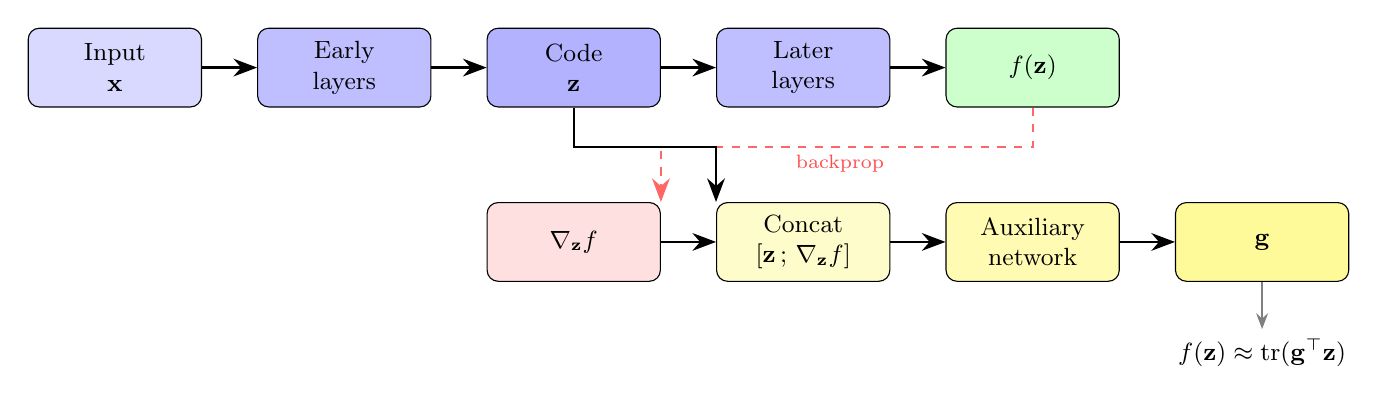
\begin{tikzpicture}[
    block/.style={draw, rounded corners, minimum height=1cm, minimum width=2.2cm,
                  align=center, font=\small},
    arr/.style={-{Stealth[length=3mm]}, thick},
    node distance=0.7cm
]

% --- Main network (top) ---
\node[block, fill=blue!15] (input) {Input\\$\mathbf{x}$};
\node[block, fill=blue!25, right=of input] (early) {Early\\layers};
\node[block, fill=blue!30, right=of early] (code) {Code\\$\mathbf{z}$};
\node[block, fill=blue!25, right=of code] (later) {Later\\layers};
\node[block, fill=green!20, right=of later] (fz) {$f(\mathbf{z})$};

\draw[arr] (input) -- (early);
\draw[arr] (early) -- (code);
\draw[arr] (code)  -- (later);
\draw[arr] (later) -- (fz);

% --- Gradient arrow ---
\node[block, fill=red!12, below=1.2cm of code] (grad) {$\nabla_{\mathbf{z}} f$};
\draw[arr, dashed, red!60] (fz.south) -- ++(0,-0.5) -| (grad.north east)
    node[pos=0.65, right=45pt, font=\scriptsize, red!70] {backprop};

% --- Auxiliary network ---
\node[block, fill=yellow!20, below=1.2cm of later] (concat) {Concat\\$[\mathbf{z} \,;\, \nabla_{\mathbf{z}} f]$};
\node[block, fill=yellow!30, right=of concat] (aux) {Auxiliary\\network};
\node[block, fill=yellow!40, right=of aux] (g) {$\mathbf{g}$};

% arrows into concat
\draw[arr] (code.south) -- ++(0,-0.5) -| (concat.north west);
\draw[arr] (grad) -- (concat);

\draw[arr] (concat) -- (aux);
\draw[arr] (aux)    -- (g);

% approximation annotation
\node[below=0.6cm of g, font=\small, align=center] (approx)
    {$f(\mathbf{z}) \approx \operatorname{tr}(\mathbf{g}^\top \mathbf{z})$};
\draw[thick, gray, -{Stealth[length=2mm]}] (g.south) -- (approx.north);

\end{tikzpicture}
\caption{Interpretation network. The auxiliary network receives the code
$\mathbf{z}$ and its gradient $\nabla_{\mathbf{z}} f$, and outputs a
pseudo-gradient $\mathbf{g}$ that linearly approximates the prediction.}
\label{fig:interp-net}
\end{figure}

The auxiliary network takes as input both $\mathbf{z}$ and the gradient
$\nabla_{\mathbf{z}} f$ (concatenated along the channel axis) and produces a
pseudo-gradient $\mathbf{g} \in \mathbb{R}^{\ell \times c}$ of the same shape
as $\mathbf{z}$.  It is trained so that the prediction network's output is
well-approximated by the linear surrogate
\begin{equation}
  f(\mathbf{z}) \;\approx\; \operatorname{tr}\!\bigl(\mathbf{g}^{\!\top}\,
  \mathbf{z}\bigr)
  \;=\; \sum_{i,j} g_{ij}\, z_{ij}\,.
\end{equation}
Because $\mathbf{g}$ has the same spatial and channel dimensions as the code,
each entry $g_{ij}$ quantifies the local importance of the corresponding feature
at position~$i$ and channel~$j$.  This provides a per-position, per-filter
attribution that can be read off directly from the learned convolutional
features, enabling downstream motif analysis without relying on post-hoc
gradient saliency alone.

\section{Prediction Network}

The prediction network is a deep neural network that maps one-hot encoded
biological sequences to scalar (or multi-output) predictions.  It combines
convolutional feature extraction with channel-wise attention, drawing on
design principles from EfficientNet~\cite{tan2019efficientnet,tan2021efficientnetv2},
and operates in two stages.

\begin{figure}[ht]
\centering

% ── Pipeline diagram (rescaled to text width) ──
\resizebox{\textwidth}{!}{%
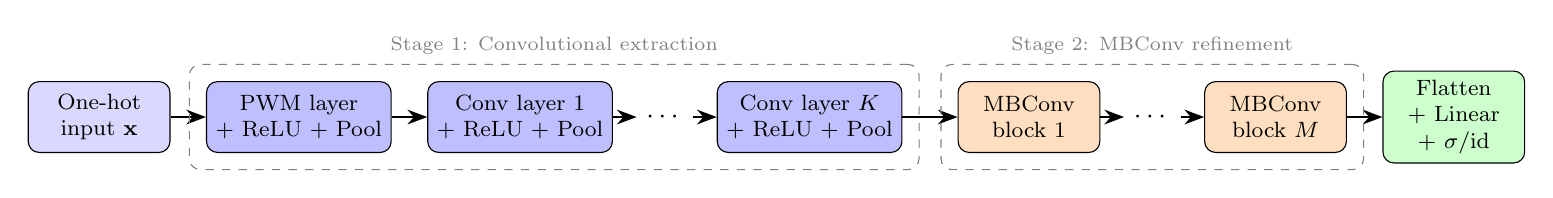
\begin{tikzpicture}[
    block/.style={draw, rounded corners, minimum height=0.9cm, minimum width=1.8cm,
                  align=center, font=\footnotesize},
    stage/.style={draw, dashed, rounded corners, inner sep=6pt, gray},
    arr/.style={-{Stealth[length=2.5mm]}, semithick},
    node distance=0.45cm
]

% --- Stage 1: Conv feature extraction ---
\node[block, fill=blue!15] (input) {One-hot\\input $\mathbf{x}$};
\node[block, fill=blue!25, right=of input] (pwm) {PWM layer\\+ ReLU + Pool};
\node[block, fill=blue!25, right=of pwm] (conv1) {Conv layer 1\\+ ReLU + Pool};
\node[right=0.3cm of conv1, font=\normalsize] (dots1) {$\cdots$};
\node[block, fill=blue!25, right=0.3cm of dots1] (convK) {Conv layer $K$\\+ ReLU + Pool};

% --- Stage 2: MBConv refinement ---
\node[block, fill=orange!25, right=0.7cm of convK] (mb1) {MBConv\\block 1};
\node[right=0.3cm of mb1, font=\normalsize] (dots2) {$\cdots$};
\node[block, fill=orange!25, right=0.3cm of dots2] (mbM) {MBConv\\block $M$};

% --- Output ---
\node[block, fill=green!20, right=of mbM] (out) {Flatten\\+ Linear\\+ $\sigma / \mathrm{id}$};

% arrows
\draw[arr] (input) -- (pwm);
\draw[arr] (pwm)   -- (conv1);
\draw[arr] (conv1) -- (dots1);
\draw[arr] (dots1) -- (convK);
\draw[arr] (convK) -- (mb1);
\draw[arr] (mb1)   -- (dots2);
\draw[arr] (dots2) -- (mbM);
\draw[arr] (mbM)   -- (out);

% stage boxes
\node[stage, fit=(pwm)(conv1)(dots1)(convK),
      label={[gray, font=\scriptsize]above:Stage 1: Convolutional extraction}] {};
\node[stage, fit=(mb1)(dots2)(mbM),
      label={[gray, font=\scriptsize]above:Stage 2: MBConv refinement}] {};

\end{tikzpicture}%
}% end resizebox

\vspace{1.8em}

% ── MBConv detail (also rescaled) ──
\resizebox{0.85\textwidth}{!}{%
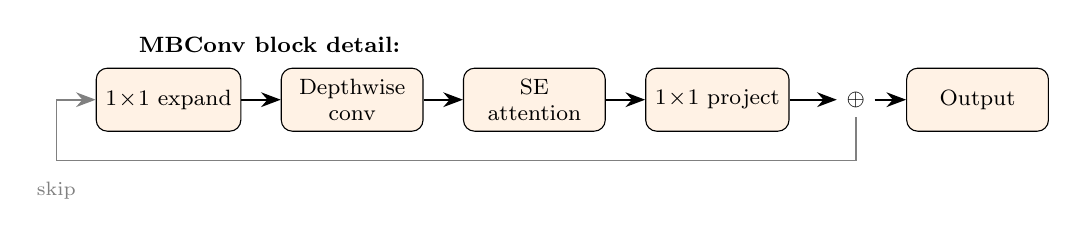
\begin{tikzpicture}[
    block/.style={draw, rounded corners, minimum height=0.8cm, minimum width=1.8cm,
                  align=center, font=\footnotesize},
    arr/.style={-{Stealth[length=2.5mm]}, semithick},
    node distance=0.5cm
]

\node[font=\footnotesize\bfseries, anchor=west] at (-0.5, 0.7) {MBConv block detail:};

\node[block, fill=orange!10] (exp) {$1\!\times\!1$ expand};
\node[block, fill=orange!10, right=of exp] (dw) {Depthwise\\conv};
\node[block, fill=orange!10, right=of dw] (se) {SE\\attention};
\node[block, fill=orange!10, right=of se] (proj) {$1\!\times\!1$ project};
\node[right=0.6cm of proj, font=\footnotesize] (plus) {$\oplus$};
\node[block, fill=orange!10, right=0.4cm of plus] (outmb) {Output};

\draw[arr] (exp) -- (dw);
\draw[arr] (dw)  -- (se);
\draw[arr] (se)  -- (proj);
\draw[arr] (proj) -- (plus);
\draw[arr] (plus) -- (outmb);

% skip connection
\coordinate (skipl) at ($(exp.west) + (-0.5, 0)$);
\draw[arr, gray] (skipl) -- (exp.west);
\draw[semithick, gray] (skipl) |- ($(plus.south) + (0,-0.55)$) -- (plus.south);
\node[font=\scriptsize, gray] at ($(skipl) + (0, -1.15)$) {skip};

\end{tikzpicture}%
}% end resizebox

\caption{Prediction network architecture. Top: overall pipeline. Bottom:
detail of each MBConv block with residual skip connection.}
\label{fig:pred-net}
\end{figure}

\paragraph{Stage 1: Convolutional feature extraction.}
The first layer consists of learnable position weight matrices (PWMs) applied
directly to the one-hot input, followed by ReLU activation and pooling.
Subsequent convolutional layers operate on the resulting feature maps with
additional pooling, progressively reducing spatial resolution while increasing
representational capacity.  All convolutional layers in this stage use standard
(non-depthwise) convolutions, so the network interacts with the raw sequence
signal immediately at its input.

\paragraph{Stage 2: MBConv refinement.}
After the feature-extraction stage, the representations pass through a series
of Mobile Inverted Bottleneck Convolution (MBConv) blocks~\cite{tan2019efficientnet}.
Each block interleaves local convolution with squeeze-and-excitation (SE)
channel attention: (i) $1\!\times\!1$ channel expansion, (ii) depthwise
convolution, (iii) SE attention that recalibrates channel responses globally,
and (iv) $1\!\times\!1$ projection back to the original channel count, with a
residual skip connection.  This hybrid convolution--attention design refines
the learned representations without substantially increasing the parameter count.
Similar architectures combining convolutional layers with channel attention have
been adopted for sequence-to-function prediction tasks and demonstrated
state-of-the-art performance~\cite{penzar2023legnet}.

\paragraph{Output layer.}
The refined feature maps are flattened into an embedding vector and projected to
the output dimension via a linear layer.  Depending on the task, the final
nonlinearity is either the identity (regression) or the element-wise sigmoid
(classification / probability outputs).

\bibliographystyle{plainnat}
\bibliography{bib}

\end{document}
